\documentclass[a4paper,12pt,openany]{book}
\usepackage{amsmath}     % Advanced math features
\usepackage{amsfonts}    % Math fonts
\usepackage{amssymb}     % Math symbols
\usepackage{graphicx}    % Including graphics
\usepackage{geometry}    % Page layout adjustments
\usepackage{fancyhdr}    % Custom headers and footers
\usepackage{titlesec}    % Title formatting
\usepackage{multicol}    % Multi-column formatting

% Page layout settings
\geometry{
  left=1in,
  right=1in,
  top=1in,
  bottom=1in,
}
% Single variable partial derivative: ∂f/∂x
\newcommand{\pd}[2]{\dfrac{\partial #1}{\partial #2}}

% Second-order mixed partial derivative: ∂²f/∂x∂y
\newcommand{\pdm}[3]{\dfrac{\partial^2 #1}{\partial #2 \partial #3}}

% Higher-order partial derivative with a specified order: ∂ⁿf/∂xⁿ
\newcommand{\pdn}[3]{\dfrac{\partial^{#1} #2}{\partial #3^{#1}}}

\newcommand{\R}{\mathbb{R}}
\newcommand{\tsp}[3]{
    \vec{#1}\vec{#2}\vec{#3}
}

\newcommand{\dotp}[2]{
    \vec{#1} \cdot \vec{#2}
}

\newcommand{\crossp}[2]{
    \vec{#1} \times \vec{#2}
}

\newcommand{\vcomponents}[4]{
    #1 = \langle #2, #3, #4 \rangle
}
\newcommand{\grad}[1]{
    \nabla #1
}
\newcommand{\uniti}{
    \hat{\iota}
}
\newcommand{\unitj}{
    \hat{\jmath}
}
\newcommand{\unitk}{
    \hat{k}
}
\newcommand{\dirder}[2]{
    #1\prime_\vec{#2}
}
\newcommand{\abs}[1]{
    \left\vert#1\right\vert
}
\newcommand{\magn}[1]{
    \left\Vert#1\right\Vert
}
\newcommand{\parenth}[1]{
    \left(#1)\right
}

% Custom header and footer
\pagestyle{fancy}
\fancyhf{}
\fancyhead[L]{Silas Kinnear} % Replace with your name
\fancyhead[C]{MATH 283}
\fancyhead[R]{\thepage}

% Title format
\titleformat{\chapter}[block]{\LARGE\bfseries}{\thechapter.}{1em}{}
\titleformat{\section}[block]{\Large\bfseries}{\thesection}{1em}{}
\titleformat{\subsection}[block]{\large\bfseries}{\thesubsection}{1em}{}

\begin{document}

\title{Calculus III - MATH 283}
\author{Silas Kinnear}
\date{Fall 2024}
\maketitle

\tableofcontents
\fancypagestyle{plain}{
  \fancyhf{}
  \fancyhead[L]{\leftmark}
  \fancyhead[R]{Kinnear \thepage}
}
\parskip=.5cm
\parindent=0cm
%-------------------------------
% Chapter 1: Elementary Functions
%-------------------------------
\chapter{Elementary Functions}

\section{Classifications}
All functions belong to specific classifications. Algebraic functions include rational functions, and rational functions consist of polynomial functions.

\begin{itemize}
    \item \textbf{Polynomial Functions}
    \begin{itemize}
        \item Addition
        \item Subtraction
        \item Multiplication
    \end{itemize}
    \item \textbf{Rational Functions}
    \begin{itemize}
        \item Division
    \end{itemize}
    \item \textbf{Algebraic Functions}
    \begin{itemize}
        \item Rational Powers
    \end{itemize}
\end{itemize}
All of these operations combined a finite number of times in one formula are known as elementary functions.

\section{Limits and Continuity}

\begin{align*}
    \lim_{x \to 0} \dfrac{1}{x} &= \infty \quad \text{(DNE)} \\
    \lim_{x \to 0^+} \ln(x) &= -\infty \quad \text{(DNE)} \\
    \lim_{x \to 0^-} \ln(x) &= \text{DNE}
\end{align*}

%-------------------------------
% Chapter 2: Dimensional Analysis
%-------------------------------
\chapter{Dimensional Analysis}

\section{Introduction}
Dimensional analysis is a fundamental tool in understanding the relationships between different physical quantities.

\section{Classifications}

\begin{align*}
    \text{Circle:} \quad & (x-h)^2 + (y-k)^2 = r^2 \\
    \text{Sphere:} \quad & (x-h)^2 + (y-k)^2 + (z-l)^2 = r^2 \\
    \text{Disk:} \quad & (x-h)^2 + (y-k)^2 \leq r^2
\end{align*}
Here we ask: How many dimensions are needed to visualize these objects? The answer depends on the number of variables in the equation.

\begin{itemize}
    \item{\textbf{Plane Lines:} 2 variables, 1 equation}
    \item{\textbf{Space Lines:} 3 variables, 2 equations}
\end{itemize}
Examples of planes:
\[
\text{xy-plane : } z = 0
\]
\[
\text{xz-plane : } y = 0
\]
\[
\text{yz-plane : } x = 0
\]
Examples of lines:
\[
\text{x-axis : }
\begin{cases}
    z = 0\\
    y = 0
\end{cases}
\]
\[
\text{y-axis : }
\begin{cases}
    x = 0\\
    z = 0
\end{cases}
\]
\[
\text{z-axis : }
\begin{cases}
    x = 0\\
    y = 0
\end{cases}
\]
\pagebreak
\section{Geometric Equations}

\subsection{Distance Between Two Points}

The distance \(d_{PQ}\) between two points \( P(x_1, y_1, z_1) \) and \( Q(x_2, y_2, z_2) \) in three-dimensional space is given by:
\begin{equation}
    d_{PQ} = \sqrt{(x_2 - x_1)^2 + (y_2 - y_1)^2 + (z_2 - z_1)^2}
\end{equation}

\subsection{Midpoint Formula}

The midpoint \(M_{PQ}\) between two points \( P(x_1, y_1, z_1) \) and \( Q(x_2, y_2, z_2) \) is calculated as:
\begin{equation}
    M_{PQ} = \left(\dfrac{x_1 + x_2}{2}, \dfrac{y_1 + y_2}{2}, \dfrac{z_1 + z_2}{2}\right)
\end{equation}

\subsection{Equation of a Sphere}

A sphere centered at \(P(p, q, s)\) with radius \( r \) has the equation:
\begin{equation}
    (x - p)^2 + (y - q)^2 + (z - s)^2 = r^2
\end{equation}

\subsection{Equation of an Ellipsoid}

An ellipsoid centered at \(P(h, k, l)\) is given by:

\begin{equation}
    \dfrac{(x-h)^2}{a^2} +  
    \dfrac{(y-k)^2}{b^2} + 
    \dfrac{(z-l)^2}{c^2} = 1
\end{equation}

\subsection{Equations of a Line}
\(\vec{a_l} = \langle a, b, c \rangle\) is the vector collinear to the line, and \(P(x_0, y_0, z_0)\) is a point on the line.
\subsubsection{Parametric Form}
\begin{equation}
    l = 
    \begin{cases}
        x = x_0 + at\\
        y = y_0 + bt\\
        z = z_0 + ct
    \end{cases}
\end{equation}

\subsubsection{Normal Form}
\begin{equation}
    \dfrac{x-x_0}{a} = \dfrac{y-y_0}{b} = \dfrac{z-z_0}{c}
\end{equation}

\subsection{Equations of a Plane}
\(\vec{a_l} = \langle a, b, c \rangle\) is the vector normal to the plane, and \(P(x_0, y_0, z_0)\) is a point on the plane.
\subsubsection{Point-Normal/Scalar Form}
\begin{equation}
    a(x-x_0) + b(y-y_0) + c(z-z_0) = 0
\end{equation}
\section{Graphing Concepts}

Graphing helps visualize functions and equations by showing the set of all points that satisfy them.

\subsection{Functions of a Single Variable}

For a function of a single variable \( f(x) \):
\begin{itemize}
    \item \textbf{Domain}: A subset or all of the real number line, often denoted as \(\mathbb{R}\) or a specific interval such as \((- \infty, \infty)\).
    \item \textbf{Range}: The set of possible values of \( f(x) \); for instance, \([0, \infty)\).
    \item \textbf{Graph}: A curve on the Cartesian plane, representing ordered pairs \((x, f(x))\).
\end{itemize}

\subsection{Functions of Multiple Variables}

For functions of two or more variables, the domain and range extend to higher dimensions:
\begin{itemize}
    \item \textbf{Domain}: The set of all points in \(\mathbb{R}^n\) (e.g., \(\mathbb{R}^2\) for a function of two variables or \(\mathbb{R}^3\) for three variables) where the function is defined.\\
        - \textbf{Entire Plane}: If the function \( f(x, y) \) is defined for all \((x, y) \in \mathbb{R}^2\).\\
        - \textbf{Portion of the Plane}: A subset of \(\mathbb{R}^2\), specified by conditions like \(x > 0\) or \(y \geq 1\) or given by a picture.
    \item \textbf{Range}: The set of output values of the function. For many functions of multiple variables, this is a subset of \(\mathbb{R}\).
    \item \textbf{Graph}: For a function \( f(x, y) \) in two variables, the graph is a surface in three-dimensional space. For functions of three variables, the graph would exist in four-dimensional space and cannot be directly visualized.
\end{itemize}

\subsection*{Examples of Functions of Multiple Variables}

\textbf{1: Linear Function of Two Variables}
    \[
    f(x, y) = 3x + 5y - 7
    \]
    \begin{itemize}
        \item \textbf{Domain}: \(\mathbb{R}^2\) (all real pairs \((x, y)\))
        \item \textbf{Range}: \(\mathbb{R}\) (all real values)
        \item \textbf{Graph}: A plane in three-dimensional space.
    \end{itemize}

\textbf{2: Linear Function of Three Variables}
    \[
    f(x, y, z) = 3x - 5y + z - 11
    \]
    \begin{itemize}
        \item \textbf{Domain}: \(\mathbb{R}^3\) (all real triples \((x, y, z)\))
        \item \textbf{Range}: \(\mathbb{R}\)
        \item \textbf{Graph}: Exists in four-dimensional space; it cannot be visualized in three dimensions.
    \end{itemize}
\textbf{3: Rational Function of Two Variables}
    \[
        f(x, y) = 5 - 7 \sqrt{13-x^2-y^2-2x}
    \]
    \begin{itemize}
        \item \textbf{Domain}: $(x-1)^2+y^2 \leq 14$, disk with center $(1, 0)$ with radius $\sqrt{14}$.
        \begin{center}
            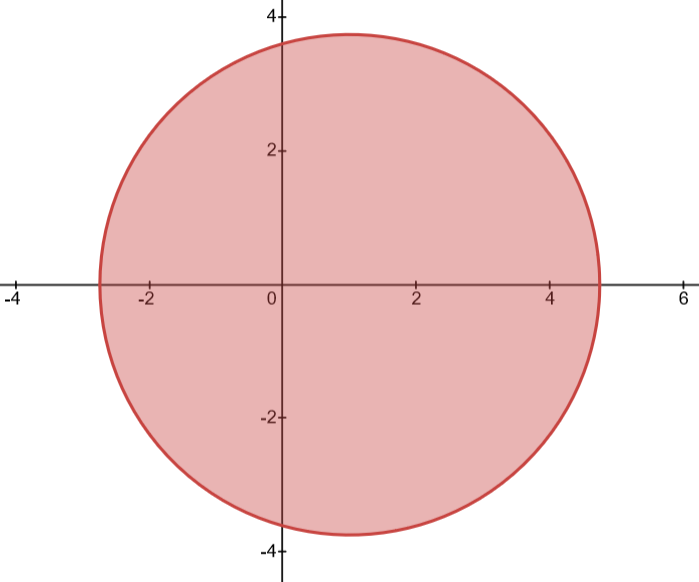
\includegraphics[width=0.3\textwidth]{domain1.png}
        \end{center}
        \item \textbf{Range}: $\left[5-7\sqrt{13}, 5\right]$
        \item \textbf{Graph}: A surface in three-dimensional space. This equation can be rewritten as 
        \[
            \dfrac{\left(x-1\right)^{2}}{14}+\dfrac{\left(y\right)^{2}}{14}+\dfrac{\left(z-5\right)^{2}}{49\cdot14}=1
        \] 
        \begin{center}
            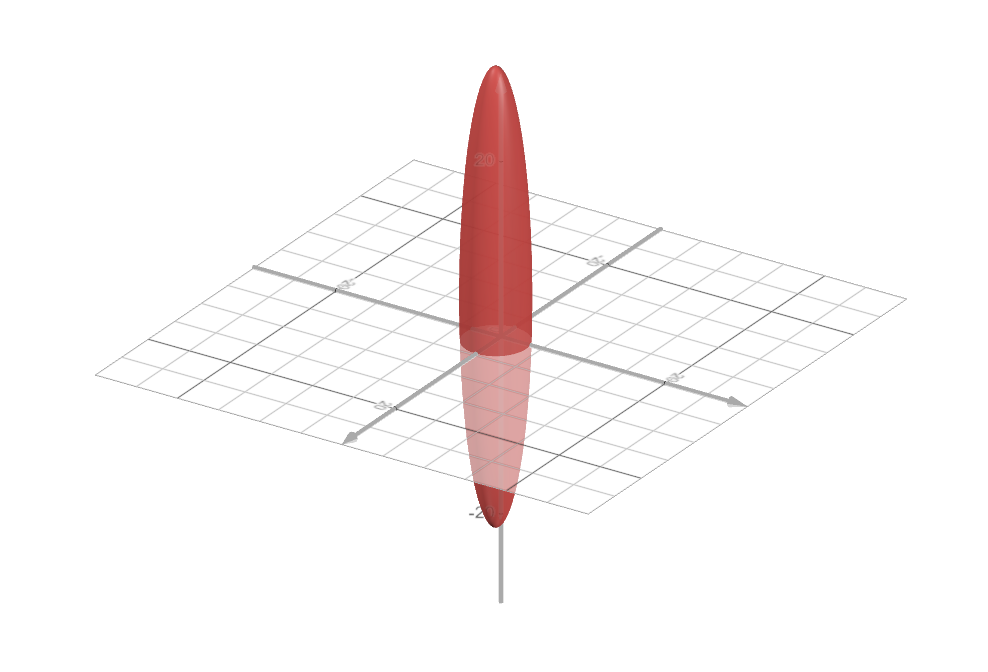
\includegraphics[width=0.5\textwidth]{graph1.png}
        \end{center}
    \end{itemize}

\textbf{4: Trigonometric Function of Two Variables}
    \[
        f(x,y) = 
        3 - \dfrac{5}{\pi}\arcsin(x+y)
    \]
    \begin{itemize}
        \item \textbf{Domain}: $-1 \leq x+y \leq 1$
        \begin{center}
            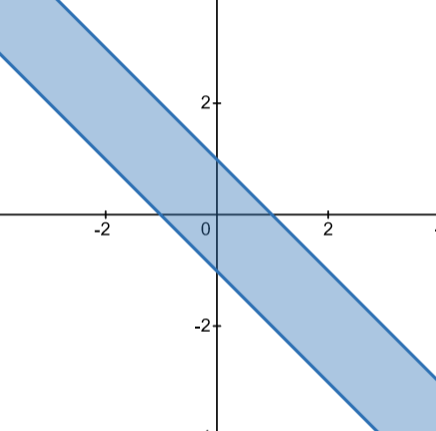
\includegraphics[width=0.3\textwidth]{domain2.png}
        \end{center}
        \item \textbf{Range}: \[\dfrac{-\pi}{2} \leq \arcsin(x+y) \leq \dfrac{\pi}{2}, \, z \in \left[\dfrac{1}{2}, \dfrac{11}{2}\right]\]
        \item \textbf{Graph}: A surface in three-dimensional space.
        \begin{center}
            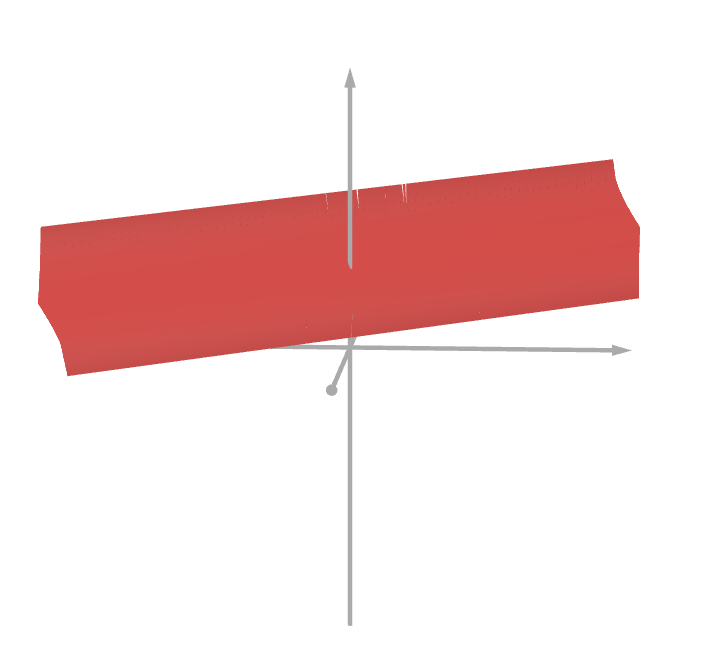
\includegraphics[width=0.5\textwidth]{graph2.png}
        \end{center}
    \end{itemize}
\section{Graphing Dimensions Summary}

Graphing dimensions change based on the variables involved:
\begin{itemize}
    \item \textbf{1D}: Interval or union of intervals
    \item \textbf{2D}: Picture
    \item \textbf{3D}: Description
    \item \textbf{4D and Higher}: Equation
\end{itemize}

%-------------------------------
% Chapter 3: Functions of Several Variables
%-------------------------------
\chapter{Functions of Several Variables}
Functions of several variables extend the concept of functions to higher dimensions, allowing for more complex mappings and dependencies.

% Example content for introduction, definitions, and properties of functions of several variables.

%-------------------------------
% Chapter 4: Partial Derivatives
%-------------------------------
\chapter{Partial Derivatives}
Partial derivatives are used to study functions with multiple variables by differentiating with respect to one variable while keeping the others constant.

\section{Differentiability}
A function of more than two variables is said to be
differentiable if the function all of its first partial
derivative and all of its second partial derivatives exist
and are continuous.

\section{Introduction}
Partial derivatives are used to study how a function changes with respect to one variable while keeping the others constant.

\subsection{Differentials}
The derivative of a function \(f(x)\) with respect to \(x\) is denoted as: $\dfrac{dy}{dx}$ or $f'(x)$ where dx is the differential of x and $dy = f'(x)dx$.
Differentials are different than derivatives, as they are the change in the function value due to a change in the variable. For example,
\[
\text{if }f(x) = x^2\text{, then } df = 2xdx\text{.}
\]
\[
d(\arctan(u)) = \dfrac{du}{1+u^2}\text{ but }\arctan(u') = \dfrac{u'}{1+u^2}
\]
\subsection{Derivatives}

\[
    f(x) \text{is differentiable iff } \lim_{h \to 0} \dfrac{f(x+h) - f(x)}{h} \text{ exists}
\]
\section{Partial Derivatives}
\subsection{Partial Derivatives Definition}

The partial derivative of a function \(f(x, y)\) with respect to \(x\) is denoted as:
\[
    \pd{f}{x} = \lim_{h \to 0} \dfrac{f(x+h, y) - f(x, y)}{h}
\]
This \textbf{not} a fraction. $\partial x$ does not exist, and neither does $\partial f$.

\begin{equation}
    \pd{f}{x}(x_0, y_0) = 
    \lim_{x \to x_0} \dfrac{f(x, y_0) - f(x_0, y_0)}{x-x_0}
\end{equation}
\begin{equation}
    \pd{f}{x} = \lim_{h \to 0} \dfrac{f(x+h, y) - f(x, y)}{h}
\end{equation}
\begin{equation}
    \pd{f}{y} = \lim_{h \to 0} \dfrac{f(x, y+h) - f(x, y)}{h}
\end{equation}

\subsubsection{Shortcut}
The partial derivative of a function \(f(x, y, \cdots)\) with respect to \(x\) can be calculated by treating all other variables as a constant and differentiating with respect to \(x\):

\subsection{All Defintions of First and Second Partial Derivatives}
You sometimes have to use the definition of a partial derivative to find the actual value of the partial derivative. 
\begin{equation}
    f_x = \pd{f}{x} = \lim_{h \to 0} \dfrac{f(x+h, y) - f(x, y)}{h}
\end{equation}
\begin{equation}
    f_y = \pd{f}{y} = \lim_{h \to 0} \dfrac{f(x, y+h) - f(x, y)}{h}
\end{equation}
\begin{equation}
    f_{xy} = \pdm{f}{x}{y} = \lim_{h \to 0} \dfrac{\pd{f}{y}(x+h, y) - \pd{f}{y}(x, y)}{h}
\end{equation}
\begin{equation}
    f_{yx} = \pdm{f}{y}{x} = \lim_{h \to 0} \dfrac{\pd{f}{x}(x, y+h) - \pd{f}{x}(x, y)}{h}
\end{equation}
\begin{equation}
    f_{xx} = \pdm{f}{x}{x} = \lim_{h \to 0} \dfrac{\pd{f}{x}(x+h, y) - \pd{f}{x}(x, y)}{h}
\end{equation}
\begin{equation}
    f_{yy} = \pdm{f}{y}{y} = \lim_{h \to 0} \dfrac{\pd{f}{y}(x, y+h) - \pd{f}{y}(x, y)}{h}
\end{equation}

\subsection{Properties of Partial Derivatives}
If $f(x,y)$ is continuous at $(x_0, y_0)$, then $f_x$ and $f_y$ exist at $(x_0, y_0)$ and $f_{xy} = f_{yx}$.

\subsubsection{Total Differential}
The total differential of a function \(f(x, y)\) is given by:
\[
    df = \pd{f}{x}dx + \pd{f}{y}dy
\]
If you find df, it is very easy to find both partial derivatives via the coefficients of dx and dy.
\subsection{Higher-Order Partial Derivatives}
The second-order partial derivative of a function \(f(x, y)\) with respect to \(x\) and \(y\) is denoted as:
\[
    \pdm{f}{x}{y} = \pd{}{x}\left(\pd{f}{y}\right)
\]
Order does matter. For example, for some instances: \[\pdm{f}{x}{y} \neq \pdm{f}{y}{x}\] However, these are usually equal for continuous functions. It is read from left to right and can also be notated as \(f_{xy}\) or \(f_{xy}\).
\pagebreak
\section{Examples:}
\[
    f(x, y) = 
    \begin{cases}
        \dfrac{x^2 y}{x^2 + y^2}, & (x, y) \neq (0, 0)\\
        0, & (x, y) = (0, 0)
    \end{cases}
\]

For \( (x, y) \neq (0, 0) \), the partial derivatives are:
\[
    \pd{f}{x} = \dfrac{2xy^3}{(x^2 + y^2)^2}
\]
\[
    \pd{f}{y} = \dfrac{x^4 - x^2 y^2}{(x^2 + y^2)^2}
\]
\[
    \pdm{f}{x}{y} = \dfrac{2x^3 y^2 - 2x y^4}{(x^2 + y^2)^3}
\]
\[
    \pdm{f}{y}{x} = \dfrac{2x^3 y^2 - 2x y^4}{(x^2 + y^2)^3}
\]
\[
    \pdm{f}{x}{x} = \dfrac{2y^3(x^2 - y^2)}{(x^2 + y^2)^3}
\]
\[
    \pdm{f}{y}{y} = \dfrac{x^2(2x^2 - y^2)}{(x^2 + y^2)^3}
\]

For \( (x, y) = (0, 0) \), we use the limit definition of partial derivatives. The partial derivative of \( f \) with respect to \( x \) at \( (0, 0) \) is:
\[
    \pd{f}{x}(0, 0) = \lim_{h \to 0} \dfrac{f(h, 0) - f(0, 0)}{h} = \lim_{h \to 0} \dfrac{0 - 0}{h} = 0
\]
Similarly, the partial derivative of \( f \) with respect to \( y \) at \( (0, 0) \) is:
\[
    \pd{f}{y}(0, 0) = \lim_{k \to 0} \dfrac{f(0, k) - f(0, 0)}{k} = \lim_{k \to 0} \dfrac{0 - 0}{k} = 0
\]

Thus, we have:
\[
    \pd{f}{x}(0, 0) = 0, \quad \pd{f}{y}(0, 0) = 0
\]

To find the second partial derivatives at \( (0, 0) \), we proceed similarly:
\[
    \pdm{f}{x}{x}(0, 0) = \lim_{h \to 0} \dfrac{\pd{f}{x}(h, 0) - \pd{f}{x}(0, 0)}{h} = \lim_{h \to 0} \dfrac{0 - 0}{h} = 0
\]
\[
    \pdm{f}{y}{y}(0, 0) = \lim_{k \to 0} \dfrac{\pd{f}{y}(0, k) - \pd{f}{y}(0, 0)}{k} = \lim_{k \to 0} \dfrac{0 - 0}{k} = 0
\]
\[
    \pdm{f}{x}{y}(0, 0) = \pdm{f}{y}{x}(0, 0) = \lim_{h \to 0} \dfrac{\pd{f}{y}(h, 0) - \pd{f}{y}(0, 0)}{h} = 0
\]

Thus, all second partial derivatives at \( (0, 0) \) are:
\[
    \pdm{f}{x}{x}(0, 0) = 0, \quad \pdm{f}{y}{y}(0, 0) = 0, \quad \pdm{f}{x}{y}(0, 0) = 0, \pdm{f}{y}{x}(0, 0) = DNE
\]
\[
    \pdm{f}{y}{x}(0, 0) = 
    \lim_{x\to 0} \dfrac{\pd{f}{x}(x, 0) - \pd{f}{x}(0, 0)}{x} = \lim_{x\to 0} \dfrac{1 - 0}{x} = DNE
\]

All partial derviatives combined are:
\[
    \pd{f}{x} = 
    \begin{cases}
        \dfrac{2xy^3}{(x^2 + y^2)^2}, & (x, y) \neq (0, 0)\\
        0, & (x, y) = (0, 0)
    \end{cases}
\]
\[
    \pd{f}{y} = 
    \begin{cases}
        \dfrac{x^4 - x^2 y^2}{(x^2 + y^2)^2}, & (x, y) \neq (0, 0)\\
        0, & (x, y) = (0, 0)
    \end{cases}
\]
\[
    \pdm{f}{x}{y} = 
    \begin{cases}
        \dfrac{2x^3 y^2 - 2x y^4}{(x^2 + y^2)^3}, & (x, y) \neq (0, 0)\\
        0, & (x, y) = (0, 0)
    \end{cases}
\]
\[
    \pdm{f}{y}{x} = 
    \begin{cases}
        \dfrac{2x^3 y^2 - 2x y^4}{(x^2 + y^2)^3}, & (x, y) \neq (0, 0)\\
        DNE, & (x, y) = (0, 0)
    \end{cases}
\]
\[
    \pdm{f}{x}{x} = 
    \begin{cases}
        \dfrac{2y^3(x^2 - y^2)}{(x^2 + y^2)^3}, & (x, y) \neq (0, 0)\\
        0, & (x, y) = (0, 0)
    \end{cases}
\]
\[
    \pdm{f}{y}{y} = 
    \begin{cases}
        \dfrac{x^2(2x^2 - y^2)}{(x^2 + y^2)^3}, & (x, y) \neq (0, 0)\\
        0, & (x, y) = (0, 0)
    \end{cases}
\]

% Example content for partial derivative rules, examples, and applications.

%-------------------------------
% Chapter 5: Multiple Integrals
%-------------------------------
\chapter{Multiple Integrals}
Multiple integrals extend single-variable integration to functions of several variables, useful in areas such as volume and area calculations.

% Example content for double and triple integrals, as well as change of variables.

%-------------------------------
% Chapter 6: Vector Calculus
%-------------------------------
\chapter{Vector Calculus}
Vector calculus explores vector fields and operations such as the gradient, divergence, and curl, which are foundational in physics, engineering, and mathematics.

\section{Introduction to Vectors and Scalars}
In mathematics and physics, \textbf{scalars} and \textbf{vectors} are fundamental quantities that describe different types of quantities.

\textbf{Scalars} are single numbers that represent quantities that have only magnitude, without any direction. Examples of scalars include:

- Temperature (e.g., \(25^\circ \text{C}\))\\
- Mass (e.g., \(5 \, \text{kg}\))\\
- Distance (e.g., \(10 \, \text{m}\))

\textbf{Vectors}, on the other hand, are quantities that have both magnitude and direction. Vectors are represented as an ordered list of components in a coordinate system. For example, in three-dimensional space, a vector \(\vec{v}\) can be represented as:
\[
\vec{v} = \langle v_x, v_y, v_z \rangle.
\]
An example of a vector is a displacement of \(5 \, \text{m}\) to the right and \(3 \, \text{m}\) upwards, represented as \(\vec{d} = \langle 5, 3, 0 \rangle\).

In summary:

- A \textbf{scalar} is a quantity that has only magnitude.\\
- A \textbf{vector} is a quantity that has both magnitude and direction.

\subsection{Vector Addition}
You \textbf{cannot} add a vector and a scalar. However, you can add two vectors together. Vector addition combines two vectors \(\vec{u}\) and \(\vec{v}\) to produce a resultant vector \(\vec{w}\):
\[
    \vec{w} = \vec{u} + \vec{v} = \langle u_x + v_x, u_y + v_y, u_z + v_z \rangle
\]
For example, given these vectors: $\vcomponents{u}{1}{2}{3}$, and $\vcomponents{v}{4}{5}{6}$
\[
\vec{u} + \vec{v} = \langle 1 + 4, 2 + 5, 3 + 6 \rangle = \langle 5, 7, 9 \rangle
\]

\subsection{Vector Scalar Multiplication}
A vector and scalar can be multiplied, but two vectors cannot be multiplied in the traditional sense.
\[
    k\vec{u} = \langle ku_x, ku_y, ku_z \rangle
\]


\subsection{Scalar Multiples}
A scalar multiple of a vector \(\vec{u}\) scales its magnitude without changing its direction. If \(\vec{v}\) is collinear to \(\vec{u}\), then there exists some scalar $k$ where \(\vec{v} = k\vec{u}\).
For example, given these vectors: $\vcomponents{u}{1}{2}{3}$, and $\vcomponents{v}{2}{4}{6}$
\[
2\vec{u} = \vec{v}
\]
\[
2\left\langle 1, 2, 3\right\rangle = 
\left\langle 2, 4, 6\right\rangle
\]
For any \(\vec{u}\), \(\vec{v}\), and scalar \(k\):
\[
k\vec{u} = \langle ku_x, ku_y, ku_z \rangle
\]
\[
    \text{iff } \vec{v} = \langle ku_x, ku_y, ku_z \rangle \text{ for some scalar } k, \vec{v} \parallel \vec{u}
\]


\section{Dot Product}
The dot product is an operation between two vectors \(\vec{u}\) and \(\vec{v}\) that produces a scalar, and is calculated as:
\[
    \vec{u} \cdot \vec{v} = u_x v_x + u_y v_y + \cdots + u_n v_n = ||\vec{u}|| \, ||\vec{v}|| \cos{\theta}
\]
where \(\theta\) is the angle between \(\vec{u}\) and \(\vec{v}\). The dot product is \textbf{commutative}:
\[
    \vec{u} \cdot \vec{v} = \vec{v} \cdot \vec{u}
\] 

\subsection{Applications of the Dot Product}
\begin{enumerate}
    \item \textbf{Magnitude of a Vector}:
    \[
        \vec{a} \cdot \vec{a} = ||\vec{a}||^2
    \]
    \[
        ||\vec{a}|| = \sqrt{\vec{a} \cdot \vec{a}}
    \]

    \item \textbf{Determining Perpendicularity}:
    \[
        \vec{a} \cdot \vec{b} = 0 \iff \vec{a} \perp \vec{b}
    \]
    For example, if \(\vec{a}_{L_1} \cdot \vec{a}_{L_2} = 0\), then lines \(L_1\) and \(L_2\) are perpendicular.
\end{enumerate}

\section{Cross Product}
The cross product is an operation on two 3D vectors that yields a vector perpendicular to both:
\[
    \vec{u} \times \vec{v} = 
    \begin{vmatrix}
        \uniti & \unitj & \unitk \\
        u_x & u_y & u_z \\
        v_x & v_y & v_z \\
    \end{vmatrix} 
    = \langle u_y v_z - u_z v_y, \; u_z v_x - u_x v_z, \; u_x v_y - u_y v_x \rangle
\]
This resultant vector \(\vec{w} = \vec{u} \times \vec{v}\) is perpendicular to both \(\vec{u}\) and \(\vec{v}\).
\subsection{Shortcut for Cross Product}

To find the cross product \(\vec{u} \times \vec{v}\), arrange the components as follows:
\[
\begin{array}{|cccccc|}
    u_x & u_y & u_z & u_x & u_y & u_z \\
    v_x & v_y & v_z & v_x & v_y & v_z \\
\end{array}
\]

Then, calculate each component of the cross product by making crosses between $u_y$ and $v_z$, $u_z$ and $v_y$, $u_z$ and $v_x$, $u_x$ and $v_z$, $u_x$ and $v_y$, and $u_y$ and $v_x$. This yields the components of the cross product vector and is easy to visualize.

\section{Triple Scalar Product}
The triple scalar product of three vectors \(\vec{u}\), \(\vec{v}\), and \(\vec{w}\) is defined as:
\[
    \vec{u} \cdot (\vec{v} \times \vec{w}) = \vec{v} \cdot (\vec{w} \times \vec{u}) = \vec{w} \cdot (\vec{u} \times \vec{v})
\]
It is often shown as $\tsp{u}{v}{w}$ and has a few niche uses.
\begin{itemize}
    \item The volume of a parallelepiped with sides \(\vec{u}\), \(\vec{v}\), and \(\vec{w}\).
    \item The determinant of a matrix.
    \[\text{det}(M) = 
    \begin{vmatrix}
        u_x & u_y & u_z \\
        v_x & v_y & v_z \\
        w_x & w_y & w_z \\
    \end{vmatrix}
        = \tsp{u}{v}{w}
    \]
    \item The volume of a tetrahedron with noncoplanar edges \(\vec{u}\), \(\vec{v}\), and \(\vec{w}\)
        \[
            \abs{\dfrac{\tsp{u}{v}{w}}{6}}
        \]
    \item The scalar triple product is zero if the vectors are coplanar. 
        \[
            \text{iff }\, \tsp{u}{v}{w} = 0 \text{ then } \vec{u}, \vec{v}, \vec{w} \text{ are coplanar}
        \]
\end{itemize}
\section{Directional Derivatives}
\subsection{Definition}
The directional derivative of \(f\) at a point \((x_0, y_0, z_0)\) in the direction of a vector \(\vec{v}\) is defined as:
\[
    f'_{\vec{v}}(x_0, y_0, z_0) = 
    \lim_{h \to 0}
    \dfrac{
        f(x_0 + h \cos \alpha, y_0 + h \cos \beta, z_0 + h \cos \gamma) - f(x_0, y_0, z_0)
    }{h}
\]
\[
    f'_{\vec{v}}(x_0, y_0, z_0) = 
    \lim_{h \to 0}
    \dfrac{
        f((x_0, y_0, z_0) + h\dfrac{\vec{v}}{\magn{\vec{v}}}) - f(x_0, y_0, z_0)}{h}
\]
where \(\cos \alpha\), \(\cos \beta\), and \(\cos \gamma\) are the \textbf{directional cosines} of \(\vec{v}\).

\subsection{Shortcut Formula for Directional Derivative}
Using the gradient, the directional derivative can be computed as:
\[
    f'_{\vec{v}}(x_0, y_0, z_0) = \vec{u} \cdot \nabla f(x_0, y_0, z_0)
\]
where:
\[
    \nabla f = \left\langle \dfrac{\partial f}{\partial x}, \dfrac{\partial f}{\partial y}, \dfrac{\partial f}{\partial z} \right\rangle
\]
The gradient vector, \(\nabla f\), points in the direction of greatest increase of \(f\) and has a magnitude equal to the maximum rate of increase.

\end{document}
